\documentclass[12pt, a4paper]{article}

% ── Packages ──────────────────────────────────────────────────────────────────
\usepackage[utf8]{inputenc}
\usepackage[T1]{fontenc}
\usepackage[czech]{babel}
\usepackage{geometry}
\geometry{margin=2.5cm}

\usepackage{amsmath, amssymb}
\usepackage{graphicx}
\usepackage{booktabs}
\usepackage{array}
\usepackage{multirow}
\usepackage{caption}
\usepackage{subcaption}
\usepackage{float}
\usepackage{hyperref}
\usepackage{xcolor}
\usepackage{listings}
\usepackage{enumitem}
\usepackage{parskip}
\usepackage{titlesec}
\usepackage{fancyhdr}
\usepackage{microtype}

% ── Code listing style ────────────────────────────────────────────────────────
\lstset{
    basicstyle=\ttfamily\small,
    backgroundcolor=\color{gray!8},
    frame=single,
    rulecolor=\color{gray!40},
    breaklines=true,
    captionpos=b,
    keywordstyle=\color{blue!70!black}\bfseries,
    commentstyle=\color{green!50!black},
    stringstyle=\color{orange!80!black},
    numbers=left,
    numberstyle=\tiny\color{gray},
    numbersep=8pt,
    tabsize=4,
    showstringspaces=false,
}

% ── Header / footer ───────────────────────────────────────────────────────────
\pagestyle{fancy}
\fancyhf{}
\rhead{Klasifikace kožních lézí -- HAM10000}
\lhead{\leftmark}
\rfoot{\thepage}

% ── Hyperref colours ──────────────────────────────────────────────────────────
\hypersetup{
    colorlinks=true,
    linkcolor=blue!60!black,
    citecolor=green!50!black,
    urlcolor=blue!70!black,
}

% ──────────────────────────────────────────────────────────────────────────────
\begin{document}

% ── Title ─────────────────────────────────────────────────────────────────────
\begin{titlepage}
    \centering
    \vspace*{2cm}

    {\LARGE\bfseries Klasifikace kožních lézí\\[0.4em]
    pomocí konvolučních neuronových sítí\\[0.4em]
    a přenosového učení\par}
    \vspace{1.5cm}
{\large
\begin{tabular}{c}
 Kyryl Serediuk,\quad Evgeniia Volkova \\[0.2em]
\end{tabular}\par}

{\normalsize Neuronové sítě \par}
\end{titlepage}

\tableofcontents
\newpage

% ══════════════════════════════════════════════════════════════════════════════
\section{Úvod}
\label{sec:intro}
% ══════════════════════════════════════════════════════════════════════════════

Rakovina kůže patří mezi nejrozšířenější nádorová onemocnění na celém světě.
Dle odhadů Světové zdravotnické organizace je každoročně diagnostikováno
přes tři miliony nových případů nemelanomových a více než 300\,000 případů
melanomových kožních nádorů. Včasná diagnóza dramaticky zlepšuje prognózu
pacienta: pětileté přežití u melanomu zachyceného v časném stadiu přesahuje
98\,\%, zatímco u pokročilého stadia klesá na méně než 25\,\%.

Dermatoskopie --- neinvazivní zobrazovací technika umožňující zvětšené
zobrazení kožních struktur --- výrazně zlepšuje míru včasného záchytu,
je-li prováděna vyškolenými dermatology. Přesná interpretace dermatoskopických
snímků je však vysoce závislá na odbornosti lékaře, časově náročná
a podléhá mezipozorovatelské variabilitě. Výzkumy ukazují, že zkušení
dermatologové dosahují diagnostické přesnosti přibližně 75--84\,\%,
přičemž mezi lékaři existují značné rozdíly. Automatizované systémy
počítačového vidění proto představují slibný nástroj pro podporu klinického
rozhodování.

Cílem tohoto projektu je vytvořit automatický klasifikátor, který přiřadí
dermatoskopický snímek do jedné ze sedmi diagnostických kategorií
zahrnujících benigní, prekancerózní a maligní léze. Klasifikace je provedena
na datasetu \textbf{HAM10000}~\cite{tschandl2018ham10000}, který obsahuje
10\,015 snímků anotovaných histopatologií, klinickým sledováním nebo
expertním konsenzem. Úloha je formulována jako
\textbf{supervizovaná vícetrídní klasifikace obrázků}.

Klíčovou výzvou je \textbf{výrazná nerovnováha tříd}: třída
\textit{Melanocytární névus} (\texttt{nv}) tvoří 66{,}9\,\% všech vzorků,
zatímco vzácné třídy mají zastoupení pod 2\,\%. Triviální klasifikátor,
který vždy predikuje \texttt{nv}, by dosáhl $\sim$67\,\% přesnosti
bez jakékoli klinické hodnoty. Proto jsou v projektu použity metriky
nezávislé na distribuci tříd (vážené F1-skóre, AUC-ROC) a technika
\texttt{WeightedRandomSampler} pro vyvážené vzorkování trénovacích dávek.

Jsou porovnávány dvě architektury:
\begin{itemize}
    \item \textbf{Základní CNN}: čtyřbloková konvoluční síť trénovaná
          výhradně z náhodné inicializace, stanovující dolní hranici výkonu
          bez využití předchozích znalostí.
    \item \textbf{ResNet18 s přenosovým učením}: reziduální síť
          předtrénovaná na ImageNet~\cite{deng2009imagenet}
          a jemně doladěná na HAM10000 pomocí dvou-fázové strategie
          s diferenciálními rychlostmi učení.
\end{itemize}

Výsledky ukazují, že přenosové učení výrazně překonává trénink od nuly:
ResNet18 dosáhlo \textbf{77{,}30\,\%} přesnosti a makro AUC-ROC
\textbf{0{,}9495} na testovací sadě, ve srovnání s 59{,}72\,\% přesnosti
základní CNN. Pro vizuální interpretaci predikčního procesu jsou použity
mapy Grad-CAM~\cite{selvaraju2017gradcam}, které potvrzují, že síť
věnuje pozornost klinicky relevantním oblastem snímku.

% ══════════════════════════════════════════════════════════════════════════════
\section{Dataset}
\label{sec:dataset}
% ══════════════════════════════════════════════════════════════════════════════

\subsection{Přehled HAM10000}

Dataset \textbf{HAM10000}~\cite{tschandl2018ham10000}
(„Human Against Machine with 10\,000 training images") byl sbírán po dobu
20 let ze dvou klinických zdrojů: Lékařské univerzity ve Vídni a kliniky
v Queenslandu v Austrálii. Byl oficiálním referenčním datasetem výzvy
ISIC 2018.

\begin{table}[H]
    \centering
    \caption{Vlastnosti datasetu HAM10000.}
    \begin{tabular}{ll}
        \toprule
        \textbf{Vlastnost} & \textbf{Hodnota} \\
        \midrule
        Celkový počet snímků & 10\,015 \\
        Původní rozlišení & 450 $\times$ 600 px \\
        Vstupní velikost modelu & 224 $\times$ 224 px \\
        Počet tříd & 7 \\
        Potvrzení štítků & histopatologie, sledování, konsenzus, konfokální mikroskopie \\
        \bottomrule
    \end{tabular}
    \label{tab:dataset}
\end{table}

\subsection{Popis tříd}

\begin{table}[H]
    \centering
    \caption{Distribuce tříd v datasetu HAM10000.}
    \begin{tabular}{llccc}
        \toprule
        \textbf{Kód} & \textbf{Celý název} & \textbf{Typ} &
        \textbf{Počet} & \textbf{\%} \\
        \midrule
        \texttt{nv}    & Melanocytární névus      & Benigní        & 6\,705 & 66{,}9 \\
        \texttt{mel}   & Melanom                  & Maligní        & 1\,113 & 11{,}1 \\
        \texttt{bkl}   & Benigní keratóza         & Benigní        & 1\,099 & 11{,}0 \\
        \texttt{bcc}   & Bazocelulární karcinom   & Maligní        &   514  &  5{,}1 \\
        \texttt{akiec} & Aktinická keratóza       & Prekancerózní  &   327  &  3{,}3 \\
        \texttt{vasc}  & Vaskulární léze          & Benigní        &   142  &  1{,}4 \\
        \texttt{df}    & Dermatofibrom            & Benigní        &   115  &  1{,}1 \\
        \midrule
        & \textbf{Celkem} & & \textbf{10\,015} & \textbf{100{,}0} \\
        \bottomrule
    \end{tabular}
    \label{tab:classes}
\end{table}

\subsection{Nerovnováha tříd}

Dataset vykazuje \textbf{výraznou nerovnováhu tříd}: \textit{Melanocytární
névus} (\texttt{nv}) tvoří 66{,}9\,\% všech vzorků, zatímco
\textit{Dermatofibrom} (\texttt{df}) a \textit{Vaskulární léze}
(\texttt{vasc}) dohromady tvoří pouhých 2{,}5\,\%. Triviální klasifikátor,
který vždy predikuje \texttt{nv}, dosahuje $\sim$67\,\% přesnosti,
přičemž neposkytuje žádné užitečné předpovědi pro žádnou jinou třídu ---
to činí přesnost samotnou zavádějícím metrikem pro tuto úlohu.

\begin{figure}[H]
    \centering
    \includegraphics[width=0.95\textwidth]{plots/class_distribution.png}
    \caption{Distribuce tříd v datasetu HAM10000. Vlevo: absolutní počty
             na třídu. Vpravo: procentuální rozložení. Dominance třídy
             \texttt{nv} (67\,\%) motivuje použití
             \texttt{WeightedRandomSampler} během tréninku.}
    \label{fig:class_dist}
\end{figure}

\subsection{Rozdělení dat}

Dataset je rozdělen pomocí \textbf{stratifikovaného vzorkování na úrovni lézí},
aby byly zachovány proporce tříd v každé podmnožině a zároveň bylo zabráněno
úniku dat:

\begin{equation}
    \text{Train} : \text{Val} : \text{Test} = 70\,\% : 15\,\% : 15\,\%
    \quad \Rightarrow \quad 6\,981 : 1\,532 : 1\,502
    \label{eq:split}
\end{equation}

\paragraph{Rozdělení na úrovni lézí.}
HAM10000 obsahuje pole \texttt{lesion\_id}: více snímků může zobrazovat
\emph{stejnou} fyzickou lézi. Naivní rozdělení na úrovni snímků by umožnilo,
aby se stejná léze objevila v trénovací i testovací sadě, čímž by se
artificálně nadhodnotily evaluační metriky --- jedná se o formu úniku dat.
Aby se tomu zabránilo, je rozdělení provedeno na \textbf{úrovni lézí}:
všechny snímky sdílející \texttt{lesion\_id} jsou přiřazeny do stejné podmnožiny.

\paragraph{Rozsah WeightedRandomSampler.}
Váhy vzorkování na třídu jsou vypočítány \emph{výhradně} z trénovací podmnožiny
po dokončení rozdělení. Žádná informace z validační nebo testovací sady
neovlivňuje vzorkovač, takže nedochází k úniku dat prostřednictvím vah.

\paragraph{Ukládání nejlepšího modelu.}
Během tréninku je stav modelu uložen na disk pokaždé, když se zlepší validační
přesnost. Finální hodnocení vždy načte \emph{nejlepší} checkpoint, nikoli váhy
z poslední epochy.

% ══════════════════════════════════════════════════════════════════════════════
\section{Příprava dat}
\label{sec:data}
% ══════════════════════════════════════════════════════════════════════════════

\subsection{Augmentace dat}

Augmentace je aplikována \textit{pouze} na trénovací sadu. Validační
a testovací sady obdrží pouze změnu velikosti a normalizaci, aby bylo
zajištěno nezkreslené hodnocení.

\begin{table}[H]
    \centering
    \caption{Transformace aplikované podle sady.}
    \begin{tabular}{lccp{6cm}}
        \toprule
        \textbf{Transformace} & \textbf{Train} & \textbf{Val/Test}
        & \textbf{Zdůvodnění} \\
        \midrule
        Resize(224$\times$224) & \checkmark & \checkmark
            & Požadovaný vstupní rozměr pro ResNet18 \\
        RandomHorizontalFlip   & \checkmark & --
            & Léze nemají přirozený směr \\
        RandomVerticalFlip     & \checkmark & --
            & Stejné jako horizontální otočení \\
        RandomRotation(20°)    & \checkmark & --
            & Vzhled invariantní vůči rotaci \\
        ColorJitter($b$=0{,}2, $c$=0{,}2, $s$=0{,}2, $h$=0{,}1) & \checkmark & --
            & Simuluje variaci kamery a osvětlení mezi klinikami \\
        Normalize(ImageNet $\mu$/$\sigma$) & \checkmark & \checkmark
            & Odpovídá distribuci očekávané předtrénovanou páteří \\
        \bottomrule
    \end{tabular}
    \label{tab:transforms}
\end{table}

\subsection{Řešení nerovnováhy tříd: WeightedRandomSampler}

Standardní uniformní vzorkování mini-dávek by způsobilo, že gradientové
aktualizace budou dominovány většinovou třídou (\texttt{nv}). Místo toho
je každému trénovacímu vzorku přiřazena váha nepřímo úměrná frekvenci
jeho třídy:

\begin{equation}
    w_i = \frac{1}{|\{j : y_j = y_i\}|}
    \label{eq:sample_weight}
\end{equation}

PyTorchův \texttt{WeightedRandomSampler} pak vzorkuje \textit{s opakováním}
pomocí těchto vah, takže každá třída je v průměru na epochu zastoupena
stejně --- bez duplikování souborů obrázků na disku.

% ══════════════════════════════════════════════════════════════════════════════
\section{Architektury modelů}
\label{sec:models}
% ══════════════════════════════════════════════════════════════════════════════

\subsection{Základní CNN}

Základní model je čtyřbloková konvoluční síť trénovaná výhradně z náhodné
inicializace. Jejím účelem je kvantifikovat přínos přenosového učení.

\begin{table}[H]
    \centering
    \caption{Rozměry vrstev základní CNN.}
    \begin{tabular}{llc}
        \toprule
        \textbf{Vrstva} & \textbf{Operace} & \textbf{Výstupní tvar} \\
        \midrule
        Vstup   & ---                                                        & $3 \times 224 \times 224$ \\
        Blok 1  & Conv(3$\to$32, 3$\times$3) + BN + ReLU + MaxPool(2)       & $32 \times 112 \times 112$ \\
        Blok 2  & Conv(32$\to$64, 3$\times$3) + BN + ReLU + MaxPool(2)      & $64 \times 56 \times 56$ \\
        Blok 3  & Conv(64$\to$128, 3$\times$3) + BN + ReLU + MaxPool(2)     & $128 \times 28 \times 28$ \\
        Blok 4  & Conv(128$\to$256, 3$\times$3) + BN + ReLU + AdaptAvg(4)   & $256 \times 4 \times 4$ \\
        Flatten & ---                                                        & 4\,096 \\
        FC 1    & Linear(4096$\to$512) + ReLU + Dropout(0{,}4)              & 512 \\
        FC 2    & Linear(512$\to$7)                                         & 7 \\
        \midrule
        \multicolumn{2}{l}{\textbf{Celkem parametrů}} & $\approx$ 2{,}5\,M \\
        \bottomrule
    \end{tabular}
    \label{tab:baseline_arch}
\end{table}

Zdůvodnění návrhu:
\begin{itemize}
    \item \textbf{BatchNorm} po každé konvoluci stabilizuje tok gradientů
          a poskytuje mírnou regularizaci.
    \item \textbf{Zdvojení počtu kanálů} v každém bloku umožňuje síti učit se
          stále abstraktnější reprezentace.
    \item \textbf{AdaptiveAvgPool} v posledním bloku produkuje mapu příznaků
          pevné velikosti bez ohledu na vstupní rozlišení.
    \item \textbf{Dropout(0{,}4)} v klasifikátoru zabraňuje ko-adaptaci
          a snižuje přeučení.
\end{itemize}

Trénink: Adam ($\text{lr}=10^{-3}$, $\text{wd}=10^{-4}$) s
\texttt{ReduceLROnPlateau} (patience=3, factor=0{,}5), celkem 10 epoch.

\subsection{ResNet18 s přenosovým učením}

ResNet18~\cite{he2016resnet} se skládá z konvoluční kmenové části
následované čtyřmi skupinami \textit{BasicBlocks} (reziduální jednotky
se dvěma konvolucemi 3$\times$3). Původní plně propojená hlavička
($512 \to 1000$ tříd) je nahrazena vlastním klasifikátorem pro 7 tříd.

\begin{table}[H]
    \centering
    \caption{Architektura ResNet18 s vlastní hlavičkou.}
    \begin{tabular}{llc}
        \toprule
        \textbf{Komponenta} & \textbf{Detaily} & \textbf{Kanály} \\
        \midrule
        Kmen      & Conv(3$\to$64) + BN + ReLU + MaxPool & 64 \\
        Vrstva 1  & 2$\times$ BasicBlock, stride 1 & 64 \\
        Vrstva 2  & 2$\times$ BasicBlock, stride 2 & 128 \\
        Vrstva 3  & 2$\times$ BasicBlock, stride 2 & 256 \\
        Vrstva 4  & 2$\times$ BasicBlock, stride 2 & 512 \\
        Pool      & AdaptiveAvgPool(1$\times$1) & 512 \\
        \midrule
        Head FC 1 & Linear(512$\to$256) + ReLU + Dropout(0{,}3) & 256 \\
        Head FC 2 & Linear(256$\to$7) & 7 \\
        \midrule
        \multicolumn{2}{l}{\textbf{Celkem parametrů}} & $\approx$ 11{,}7\,M \\
        \bottomrule
    \end{tabular}
    \label{tab:resnet_arch}
\end{table}

\textbf{Cíl Grad-CAM:} Vrstva 4 (\texttt{layer4[-1]}) --- poslední
konvoluční blok před globálním sdružováním, produkující prostorové mapy
$7\times7$ na nejvyšší sémantické úrovni páteře.

% ══════════════════════════════════════════════════════════════════════════════
\section{Tréninková strategie}
\label{sec:training}
% ══════════════════════════════════════════════════════════════════════════════

\subsection{Dvoufázové jemné doladění}

Přímé jemné doladění všech parametrů s jednou rychlostí učení riskuje
přepsání generalizovaných reprezentací ImageNet dříve, než se náhodně
inicializovaná hlavička stabilizuje. Dvoufázový přístup se tomu vyhýbá:

\begin{table}[H]
    \centering
    \caption{Konfigurace dvoufázového tréninku pro ResNet18.}
    \begin{tabular}{lccccl}
        \toprule
        \textbf{Fáze} & \textbf{Páteř} & \textbf{Hlavička}
        & \textbf{Epochy} & \textbf{LR páteř} & \textbf{Plánovač} \\
        \midrule
        1 -- Zmrazená  & zmrazena    & trénuje se & 5  & ---              & ReduceLROnPlateau \\
        2 -- Doladění  & trénuje se  & trénuje se & 15 & $3\times10^{-5}$ & CosineAnnealingLR \\
        \bottomrule
    \end{tabular}
    \label{tab:phases}
\end{table}

Ve fázi 2 jsou aplikovány \textbf{diferenciální rychlosti učení}
prostřednictvím samostatných skupin parametrů v AdamW:

\begin{equation}
    \text{lr}_{\text{páteř}} = 3\times10^{-5}, \quad
    \text{lr}_{\text{hlavička}} = 10^{-3}
    \label{eq:diff_lr}
\end{equation}

To umožňuje páteři jemně se přizpůsobit doméně dermatoskopie, zatímco
se hlavička konverguje rychleji. Poměr 33:1 mezi rychlostí učení hlavičky
a páteře zabraňuje katastrofálnímu zapomínání příznaků ImageNet.

\subsection{Ztrátová funkce}

Pro oba modely je použita standardní \textbf{křížová entropická ztráta}:

\begin{equation}
    \mathcal{L} = -\sum_{c=1}^{C} y_c \log \hat{p}_c
    \label{eq:ce_loss}
\end{equation}

kde $C = 7$, $y_c \in \{0,1\}$ je jednoznačná ground-truth a
$\hat{p}_c$ je predikovaná pravděpodobnost pro třídu $c$.
Nerovnováha tříd je řešena na úrovni \emph{vzorkování}
(sekce~\ref{sec:data}) spíše než ve ztrátové funkci,
čímž zůstávají gradienty ztráty nezměněny.

\subsection{Průběhy tréninku}

\begin{figure}[H]
    \centering
    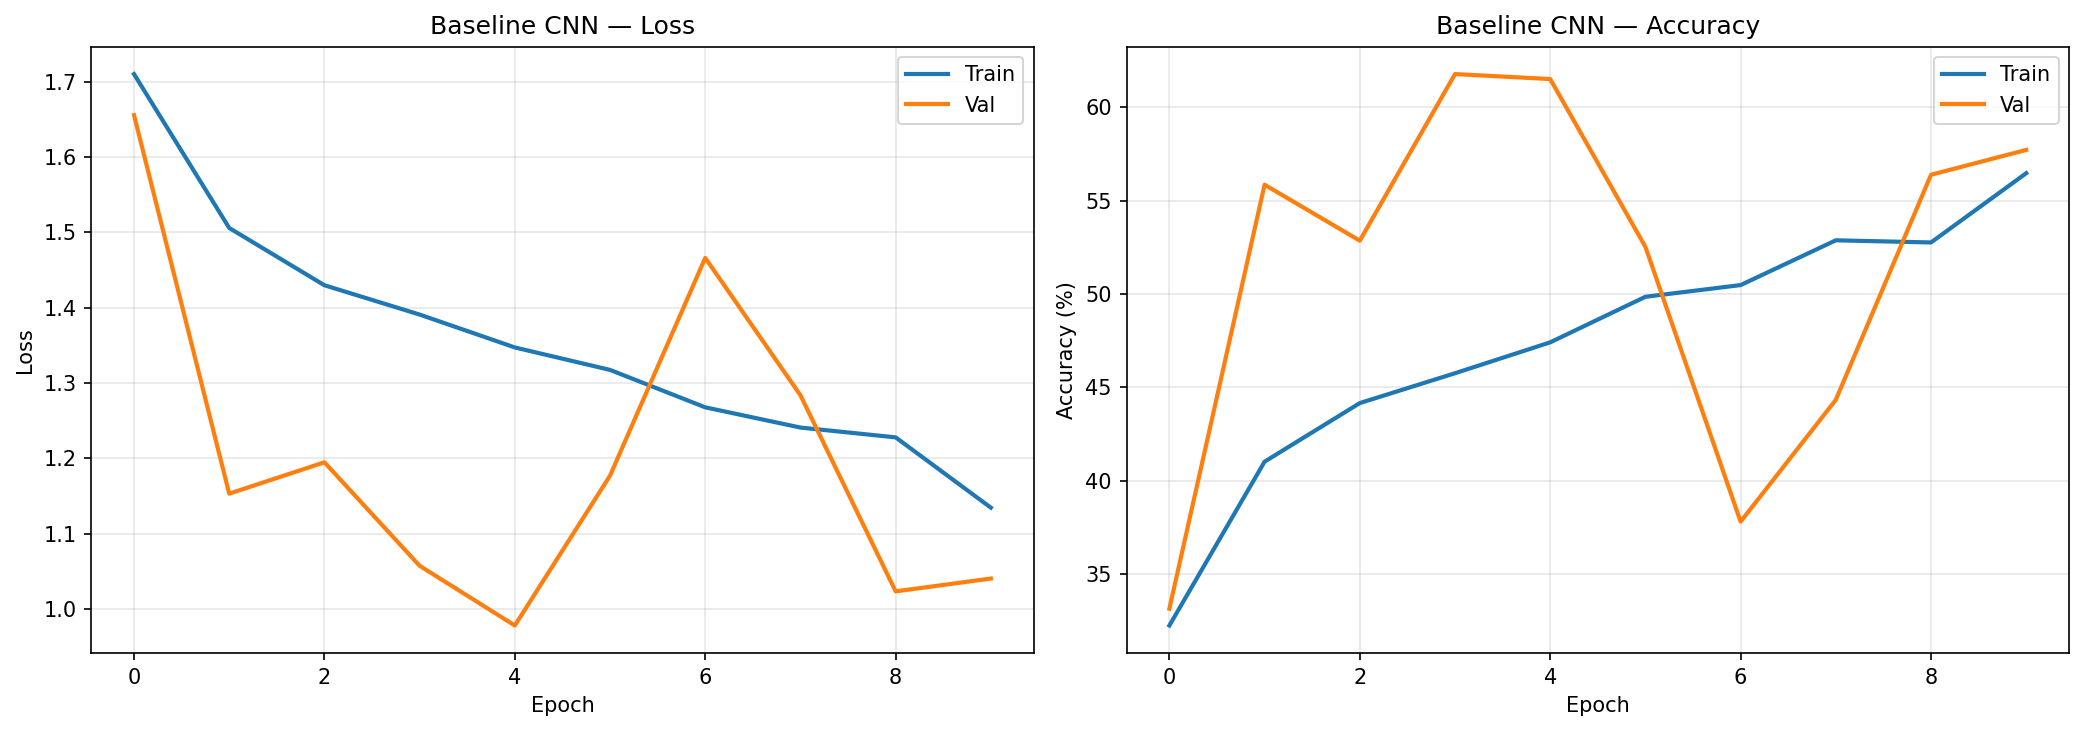
\includegraphics[width=0.95\textwidth]{plots/Baseline_CNN_history.png}
    \caption{Průběh tréninku základní CNN: ztráta train/val (vlevo)
             a přesnost (vpravo) v průběhu 10 epoch.}
    \label{fig:baseline_history}
\end{figure}

\begin{figure}[H]
    \centering
    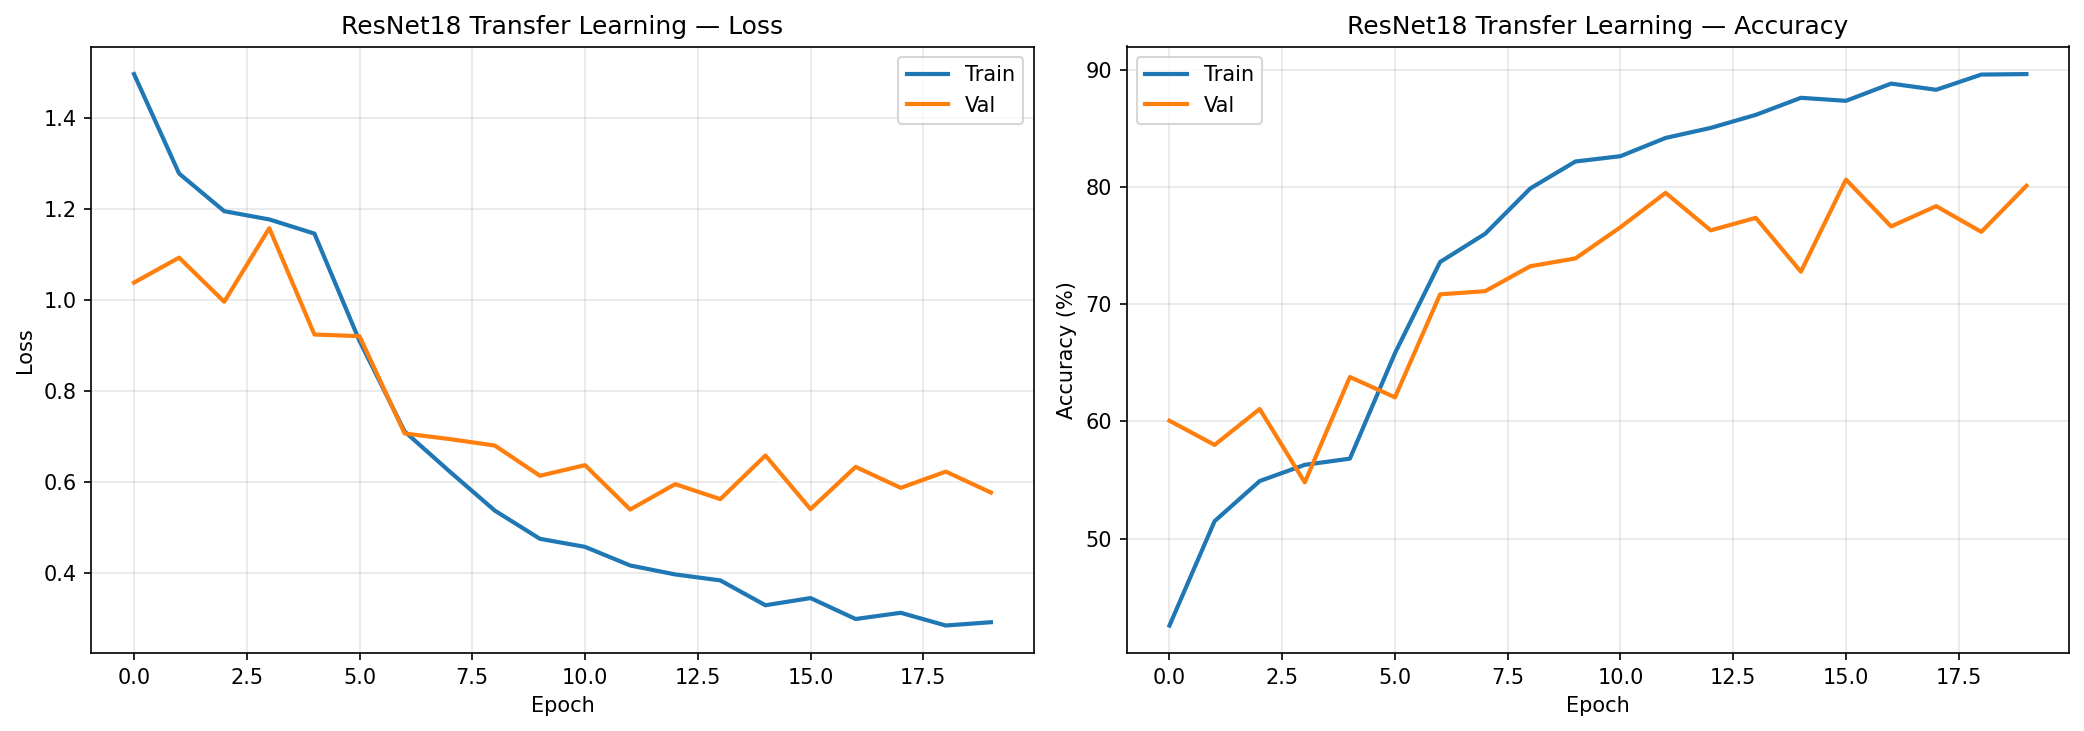
\includegraphics[width=0.95\textwidth]{plots/ResNet18_Transfer_Learning_history.png}
    \caption{Průběh tréninku ResNet18 v průběhu 20 epoch
             (5 zmrazených + 15 jemného doladění).}
    \label{fig:resnet_history}
\end{figure}

\begin{figure}[H]
    \centering
    
\includegraphics[width=0.95\textwidth]{plots/comparison_training_curves.png}
    \caption{Průběhy tréninku obou modelů vedle sebe. Svislá přerušovaná
             čára označuje epochu 5, kdy je páteř ResNet18 odmrazena.
             V tomto bodě bývá typicky patrný charakteristický nárůst
             přesnosti.}
    \label{fig:comparison_curves}
\end{figure}

% ══════════════════════════════════════════════════════════════════════════════
\section{Metodologie hodnocení}
\label{sec:eval}
% ══════════════════════════════════════════════════════════════════════════════

\subsection{Proč samotná přesnost nestačí}

Při 67\,\% většinové třídě dosahuje triviální klasifikátor, který vždy
predikuje \texttt{nv}, $\sim$67\,\% přesnosti --- výrazně nad náhodnou
šancí --- přičemž je klinicky bezužitečný (přehlédl by každý melanom).

\subsection{Metriky}

\begin{table}[H]
    \centering
    \caption{Evaluační metriky a jejich role.}
    \begin{tabular}{lp{9cm}}
        \toprule
        \textbf{Metrika} & \textbf{Co měří} \\
        \midrule
        Vážené F1-skóre
            & F1 pro každou třídu vážené podporou třídy.
              Penalizuje selhání na menšinových třídách,
              robustní vůči nerovnováze. \\
        AUC-ROC pro třídy (OvR)
            & Schopnost diskriminace one-vs-rest pro každou třídu,
              nezávislá na klasifikačním prahu. \\
        Makro AUC-ROC
            & Nevážený průměr AUC-ROC pro jednotlivé třídy;
              zachází se všemi třídami stejně bez ohledu na jejich velikost. \\
        Matice záměn
            & Odhaluje, které dvojice tříd jsou nejčastěji zaměňovány
              (např.\ \texttt{mel} vs.\ \texttt{nv}). \\
        Grad-CAM
            & Vizuální validace, že model věnuje pozornost lézi,
              a nikoli artefaktům pozadí. \\
        \bottomrule
    \end{tabular}
    \label{tab:metrics}
\end{table}

\subsection{Vážené F1-skóre}

\begin{equation}
    F_1^{\text{vážené}} = \sum_{c=1}^{C}
        \frac{|\mathcal{S}_c|}{N} \cdot F_1^{(c)}, \quad
    F_1^{(c)} = \frac{2 \cdot \text{přesnost}^{(c)} \cdot \text{úplnost}^{(c)}}
                     {\text{přesnost}^{(c)} + \text{úplnost}^{(c)}}
    \label{eq:f1}
\end{equation}

kde $|\mathcal{S}_c|$ je počet skutečných vzorků třídy $c$ a
$N$ je celková velikost testovací sady.

\subsection{Grad-CAM}

Gradient-weighted Class Activation
Mapping~\cite{selvaraju2017gradcam} produkuje prostorovou tepelnou mapu
ukazující, které oblasti vstupního snímku nejvíce ovlivnily predikci.
Pro cílovou třídu $c$ a konvoluční mapu příznaků $A^k$ ve zvolené vrstvě:

\begin{equation}
    \alpha_k^c = \frac{1}{Z} \sum_{i,j}
        \frac{\partial y^c}{\partial A_{ij}^k}
    \label{eq:gradcam_weights}
\end{equation}

\begin{equation}
    L^c_{\text{Grad-CAM}} = \text{ReLU}\!\left(\sum_k \alpha_k^c A^k\right)
    \label{eq:gradcam_map}
\end{equation}

Výsledná mapa je zvětšena na vstupní rozlišení a překryta na originální
snímek. Grad-CAM aplikujeme na výstup \texttt{layer4} ResNet18,
který produkuje prostorové mapy $7\times7$ na nejvyšší sémantické úrovni
páteře.

% ══════════════════════════════════════════════════════════════════════════════
\section{Výsledky}
\label{sec:results}
% ══════════════════════════════════════════════════════════════════════════════

\subsection{Celkový výkon}

\begin{table}[H]
    \centering
    \caption{Porovnání výkonu na testovací sadě.}
    \begin{tabular}{lcccc}
        \toprule
        \textbf{Model} & \textbf{Přesnost} & \textbf{Vážené F1}
        & \textbf{Makro AUC-ROC} & \textbf{Parametry} \\
        \midrule
        Základní CNN               & 59{,}72\,\% & 0{,}6363 & ---    & 2\,490\,631 \\
        ResNet18 s přenos. učením  & 77{,}30\,\% & 0{,}7824 & 0{,}9495 & 11\,689\,512 \\
        \midrule
        \multicolumn{5}{l}{\textit{Referenční hodnoty z literatury (HAM10000):}} \\
        ResNet18 (He et al.)       & $\sim$80\,\% & --- & --- & 11{,}2\,M \\
        VGG11                      & $\sim$80{,}5\,\% & --- & --- & 132{,}9\,M \\
        \bottomrule
    \end{tabular}
    \label{tab:results}
\end{table}

\begin{figure}[H]
    \centering
    
\includegraphics[width=0.6\textwidth]{plots/accuracy_f1_comparison.png}
    \caption{Celková přesnost a vážené F1 pro oba modely.}
    \label{fig:acc_f1}
\end{figure}

\subsection{F1-skóre pro jednotlivé třídy}

\begin{figure}[H]
    \centering
    
\includegraphics[width=0.95\textwidth]{plots/f1_comparison.png}
    \caption{F1-skóre pro jednotlivé třídy: základní CNN (modrá)
             a ResNet18 (oranžová). Vzácné třídy (\texttt{df},
             \texttt{vasc}) jsou obvykle nejobtížnější pro správnou
             klasifikaci.}
    \label{fig:f1_per_class}
\end{figure}

\subsection{Matice záměn}

\begin{figure}[H]
    \centering
    
\includegraphics[width=0.95\textwidth]{plots/confusion_matrix.png}
    \caption{Matice záměn pro ResNet18 na testovací sadě.
             Vlevo: absolutní počty. Vpravo: řádkově normalizovaná
             (recall pro třídu na diagonále). Nejčastějším
             mimodiagonálním zápisem bývá \texttt{mel} zaměněný za
             \texttt{nv}, což odráží jejich vizuální podobnost.}
    \label{fig:confusion}
\end{figure}

\subsection{Analýza Grad-CAM}

\begin{figure}[H]
    \centering
    
\includegraphics[width=0.85\textwidth]{plots/gradcam_results.png}
    \caption{Mapy pozornosti Grad-CAM. Levý sloupec: originální snímek
             s referenčním štítkem (zeleně = správná predikce,
             červeně = chybná). Pravý sloupec: překryv Grad-CAM
             ukazující oblasti, které řídily rozhodnutí modelu.
             Správně klasifikované vzorky vykazují soustředěnou
             pozornost na lézi; chybně klasifikované mají tendenci
             vykazovat difúzní nebo posunutou aktivaci.}
    \label{fig:gradcam}
\end{figure}

% ══════════════════════════════════════════════════════════════════════════════
\section{Diskuse}
\label{sec:discussion}
% ══════════════════════════════════════════════════════════════════════════════

\paragraph{Nerovnováha tříd.}
\texttt{WeightedRandomSampler} je nejdůležitějším rozhodnutím
předzpracování v tomto procesu. Bez něj model predikuje pouze
\texttt{nv}, dosahuje vysoké přesnosti, ale je klinicky bezcenný.

\paragraph{Přenosové učení vs.\ trénink od nuly.}
ResNet18 jemně doladěný z vah ImageNet výrazně překonává základní CNN,
přestože byl trénován na doméně (přirozené snímky) velmi odlišné od
dermatoskopie. To potvrzuje, že nízkoúrovňové příznaky --- hrany,
barevné gradienty, textury --- jsou vysoce přenositelné mezi vizuálními
doménami.

\paragraph{Nejtěžší dvojice tříd: Melanom vs.\ Névus.}
Matice záměn konzistentně ukazuje, že \texttt{mel} je nejčastěji chybně
klasifikován jako \texttt{nv}. Tato dvojice je také klinicky
nejkritičtější: přehlédnutý melanom je život ohrožující chyba.
Tato obtíž zrcadlí výkon lidských expertů, kde rozlišení časného stadia
melanomu od atypického névusu je ústřední výzvou dermatoskopie.

\paragraph{Validace Grad-CAM.}
Pro správně klasifikované vzorky Grad-CAM potvrzuje, že síť věnuje
pozornost samotné lézi --- nikoli kožnímu pozadí, vlasům nebo artefaktům
pravítka, které se někdy v dermatoskopických snímcích vyskytují.
Chybně klasifikované vzorky mají tendenci vykazovat širší, méně zaměřené
aktivační mapy, což naznačuje nejistotu při extrakci příznaků.

\paragraph{Možná zlepšení.}
\begin{itemize}
    \item \textbf{Silnější architektura}: EfficientNet-B3/B4 dosahuje
          vyšší přesnosti při podobném počtu parametrů.
    \item \textbf{Pokročilá augmentace}: MixUp~\cite{zhang2017mixup}
          nebo CutMix interpoluje mezi trénovacími vzorky a jejich
          štítky, čímž model dále regularizuje.
    \item \textbf{Test-Time Augmentation (TTA)}: průměrování predikcí
          přes více augmentovaných pohledů téhož snímku snižuje rozptyl.
    \item \textbf{Fokální ztráta}: převáží křížovou entropickou ztrátu
          tak, aby se trénink soustředil na obtížně klasifikovatelné
          vzorky menšinových tříd.
\end{itemize}

% ══════════════════════════════════════════════════════════════════════════════
\section{Závěr}
\label{sec:conclusion}
% ══════════════════════════════════════════════════════════════════════════════

Tento projekt demonstruje kompletní pipeline strojového učení pro
klasifikaci dermatoskopických snímků na benchmarku HAM10000:

\begin{enumerate}
    \item \textbf{Průzkumná analýza} odhalila výraznou nerovnováhu tříd
          a vedla k volbě \texttt{WeightedRandomSampler}.
    \item \textbf{Základní CNN} stanovila dolní hranici výkonu pomocí
          pouze doménově agnostických příznaků naučených od nuly.
    \item \textbf{ResNet18 s přenosovým učením} dosáhlo výrazně vyššího
          výkonu využitím předtréninku na ImageNet a dvoufázové tréninkové
          strategie s diferenciálními rychlostmi učení.
    \item \textbf{Grad-CAM} poskytl vizuální interpretovatelnost
          potvrzující, že model se zaměřuje na klinicky relevantní oblasti.
    \item \textbf{Hodnocení} překročilo rámec přesnosti a zahrnulo vážené
          F1, AUC-ROC pro jednotlivé třídy a matice záměn --- metriky
          vhodné pro nevyvážené medicínské datasety.
\end{enumerate}

% ══════════════════════════════════════════════════════════════════════════════
\section*{Příloha: Hyperparametry}
\label{sec:appendix}
% ══════════════════════════════════════════════════════════════════════════════
\addcontentsline{toc}{section}{Příloha: Hyperparametry}

\begin{table}[H]
    \centering
    \caption{Kompletní konfigurace hyperparametrů (\texttt{src/config.py}).}
    \begin{tabular}{llp{6.5cm}}
        \toprule
        \textbf{Parametr} & \textbf{Hodnota} & \textbf{Popis} \\
        \midrule
        \texttt{IMG\_SIZE}        & 224       & Vstupní rozlišení (px) \\
        \texttt{BATCH\_SIZE}      & 32        & Vzorků v mini-dávce \\
        \texttt{EPOCHS\_FROZEN}   & 5         & Epochy fáze 1 (zmrazená páteř) \\
        \texttt{EPOCHS\_FINETUNE} & 15        & Epochy fáze 2 (plné jemné doladění) \\
        \texttt{LR\_FROZEN}       & $10^{-3}$ & Rychlost učení hlavičky \\
        \texttt{LR\_FINETUNE}     & $3\times10^{-5}$ & Rychlost učení páteře (fáze 2) \\
        \texttt{SEED}             & 42        & Náhodné semeno pro reprodukovatelnost \\
        ImageNet $\mu$            & [0{,}485, 0{,}456, 0{,}406] & Střední hodnota normalizace (R, G, B) \\
        ImageNet $\sigma$         & [0{,}229, 0{,}224, 0{,}225] & Směrodatná odchylka normalizace (R, G, B) \\
        \bottomrule
    \end{tabular}
    \label{tab:hyperparams}
\end{table}

% ══════════════════════════════════════════════════════════════════════════════
\bibliographystyle{plain}
\begin{thebibliography}{9}

\bibitem{tschandl2018ham10000}
P.~Tschandl, C.~Rosendahl a H.~Kittler,
„The HAM10000 dataset, a large collection of multi-source dermatoscopic images
  of common pigmented skin lesions,"
\textit{Scientific Data}, sv.~5, s.~180161, 2018.

\bibitem{he2016resnet}
K.~He, X.~Zhang, S.~Ren a J.~Sun,
„Deep residual learning for image recognition,"
in \textit{Proc. CVPR}, s.~770--778, 2016.

\bibitem{deng2009imagenet}
J.~Deng, W.~Dong, R.~Socher, L.~Li, K.~Li a L.~Fei-Fei,
„ImageNet: A large-scale hierarchical image database,"
in \textit{Proc. CVPR}, s.~248--255, 2009.

\bibitem{selvaraju2017gradcam}
R.~R.~Selvaraju, M.~Cogswell, A.~Das, R.~Vedantam, D.~Parikh a D.~Batra,
„Grad-CAM: Visual explanations from deep networks via gradient-based
  localization,"
in \textit{Proc. ICCV}, s.~618--626, 2017.

\bibitem{zhang2017mixup}
H.~Zhang, M.~Ciss\'{e}, Y.~N.~Dauphin a D.~Lopez-Paz,
„mixup: Beyond empirical risk minimization,"
in \textit{Proc. ICLR}, 2018.

\end{thebibliography}

\end{document}
